\section{Evaluating the Classifier Performance}
\label{sec:evaluation}

During evaluation, it is essential to go beyond the loss function and consider different metrics that shed
light on various aspects of the model's performance. These metrics offer a more comprehensive understanding of how well
the classifier is doing. For example, in a binary classification problem such as diagnosing a specific medical
condition, merely looking at the loss might not reveal how well the model is identifying positive cases among the
minority class.

Classification metrics include measures like Accuracy, which gives an overall picture of correct classifications, and
Precision and Recall, which focus on the model's performance with respect to a specific class. Other metrics like the
F1-Score provide a balance between Precision and Recall, and AUC-ROC measures the ability of the model to discriminate
between positive and negative classes. Choosing the right combination of these metrics is vital, as it guides the
optimization during training and influences the model's generalization to unseen data.

Understanding and selecting the appropriate classification metrics ensures alignment with the problem's unique
requirements and goals, enhancing the model's utility and effectiveness in real-world applications.


\subsubsection{Confusion Matrix}
\label{sec:weihted-cm}

The confusion matrix provides a comprehensive view of the classifier's performance. For a binary classification task, it
is a $2\times2$ matrix where the rows correspond to the true classes and the columns correspond to the predicted classes:

\begin{equation}
    \Cbin = \begin{pmatrix}
        \text{TP} & \text{FP} \\
        \text{FN} & \text{TN} \\
    \end{pmatrix}
\end{equation}

\begin{align}
    \text{TP} & = \sum_{i=1}^{N} \llbracket y_i = 1 \land \hat{y}_i = 1 \rrbracket    \\
    \text{FP} & = \sum_{i=1}^{N} \llbracket y_i = 0 \land \hat{y}_i = 1 \rrbracket    \\
    \text{FN} & = \sum_{i=1}^{N} \llbracket y_i = 1 \land \hat{y}_i = 0 \rrbracket    \\
    \text{TN} & = \sum_{i=1}^{N} \llbracket y_i = 0 \land \hat{y}_i = 0 \rrbracket\,,
\end{align}

where TP (true positive) is the number of positive instances correctly identified as positive, TN (true negative) is the
number of negative instances correctly identified as negative, FP (false positive) is the number of negative instances
incorrectly identified as positive (Type I error), and FN (false negative) is the number of positive instances
incorrectly identified as negative (Type II error).

As explained before in the \autoref{sec:mc}, the event weights should always be used when evaluating the classifier's
performance. Otherwise, the results we obtain are not representative of the real-world performance. All of the metrics
we use thus stem from the \emph{weighted} confusion matrix, defined as:

\begin{equation}
    \Cbin_w = \begin{pmatrix}
        \text{TP}_{w} & \text{FP}_{w} \\
        \text{FN}_{w} & \text{TN}_{w} \\
    \end{pmatrix}
\end{equation}

\begin{align}
    \text{TP}_{w} & = \sum_{i=1}^{N} w_i \llbracket y_i = 1 \land \hat{y}_i = 1 \rrbracket    \\
    \text{FP}_{w} & = \sum_{i=1}^{N} w_i \llbracket y_i = 0 \land \hat{y}_i = 1 \rrbracket    \\
    \text{FN}_{w} & = \sum_{i=1}^{N} w_i \llbracket y_i = 1 \land \hat{y}_i = 0 \rrbracket    \\
    \text{TN}_{w} & = \sum_{i=1}^{N} w_i \llbracket y_i = 0 \land \hat{y}_i = 0 \rrbracket\,,
\end{align}

where $\Cbin_w$ is the confusion matrix, $w_i$ is the \gls{mc} weight of the $i$-th event, calculated as described in the
\appref{appendix:weights}, and $N$ is the total number of events in the evaluation set. Further on, when referring to
the confusion matrix, true positives, false positives, false negatives, and true negatives, we will always be referring
to their weighted counterparts, dropping the subscript $w$ for brevity, unless otherwise specified.

\autoref{fig:cm} shows how such confusion matrix looks in our case for the binary classification task - when we only
care about differentiating between \tth and non-\tth events.

\begin{figure}[htb]
    \centering
    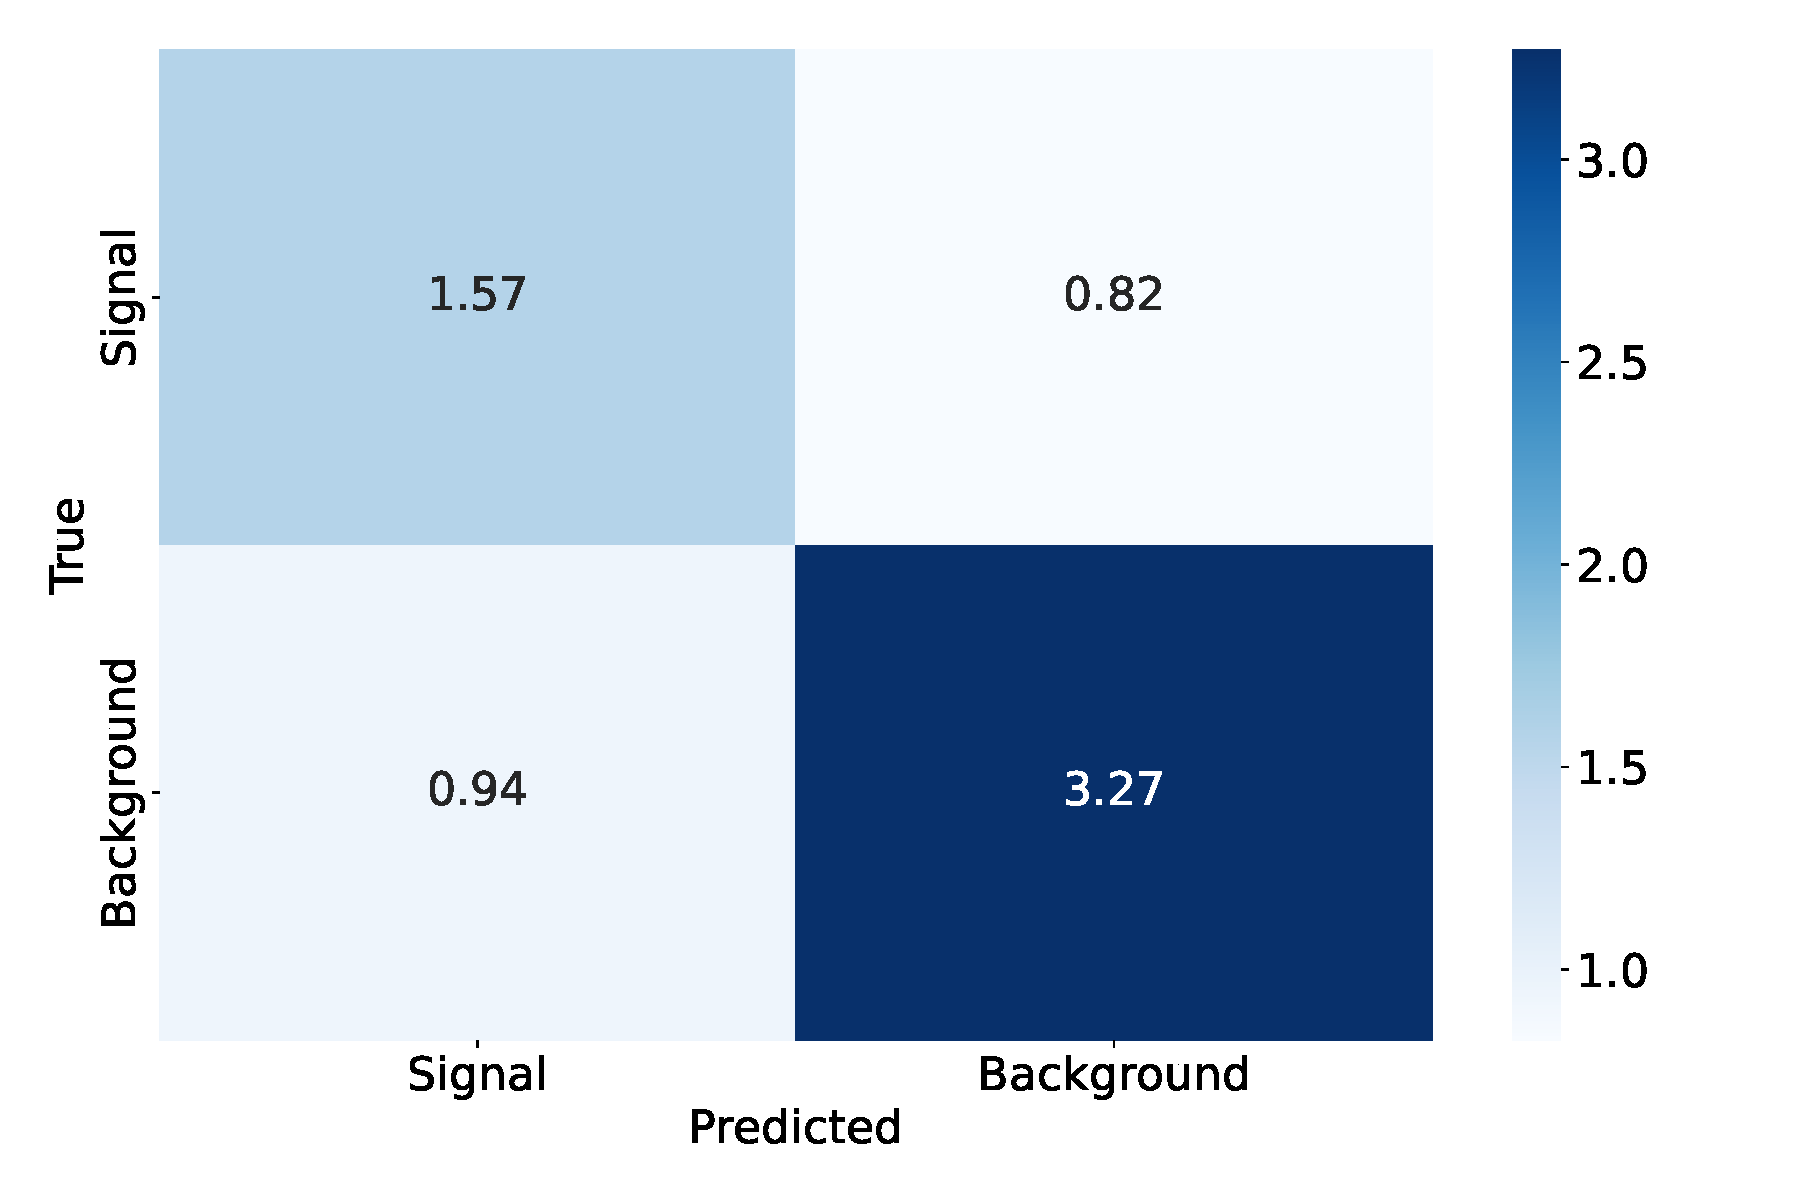
\includegraphics[trim=0.5cm 0 3cm 0, clip, width=0.8\textwidth]{figures/ml/cm/signal_argmax.pdf}
    \caption[Confusion matrix for a binary classification task]
    {Confusion matrix for a binary classification task. This confusion matrix is produced using 5-blocks
        \gls{ftt} (see \autoref{sec:ftt}) trained on the extended training set (see \autoref{sec:extended-set}). The
        $\arg\max$ classification strategy was used.  Note that the classifier was \emph{trained} to differentiate
        between all the classes, but during evaluation, all the non-\tth events are grouped together.}
    \label{fig:cm}
\end{figure}

Binary confusion matrix naturally extends to a multi-class formulation (\autoref{fig:cm-muli}), leading to a
$|\classY| \times |\classY|$ matrix for an $|\classY|$-class classification task:

\begin{equation}
    \Cmulti_{ij} = \sum_{k=1}^{|\classY|} w_k \llbracket y_k = i \land \hat{y}_k = j \rrbracket\,,
\end{equation}

where $i$ and $j$ are the true and predicted classes, respectively. The diagonal elements of the matrix correspond to
the correctly classified events, while the off-diagonal elements correspond to the misclassified events. The
multi-class confusion matrix is not symmetric, and the sum of the elements in each row is equal to the number of events
in the corresponding true class.

\begin{figure}[htb]
    \centering
    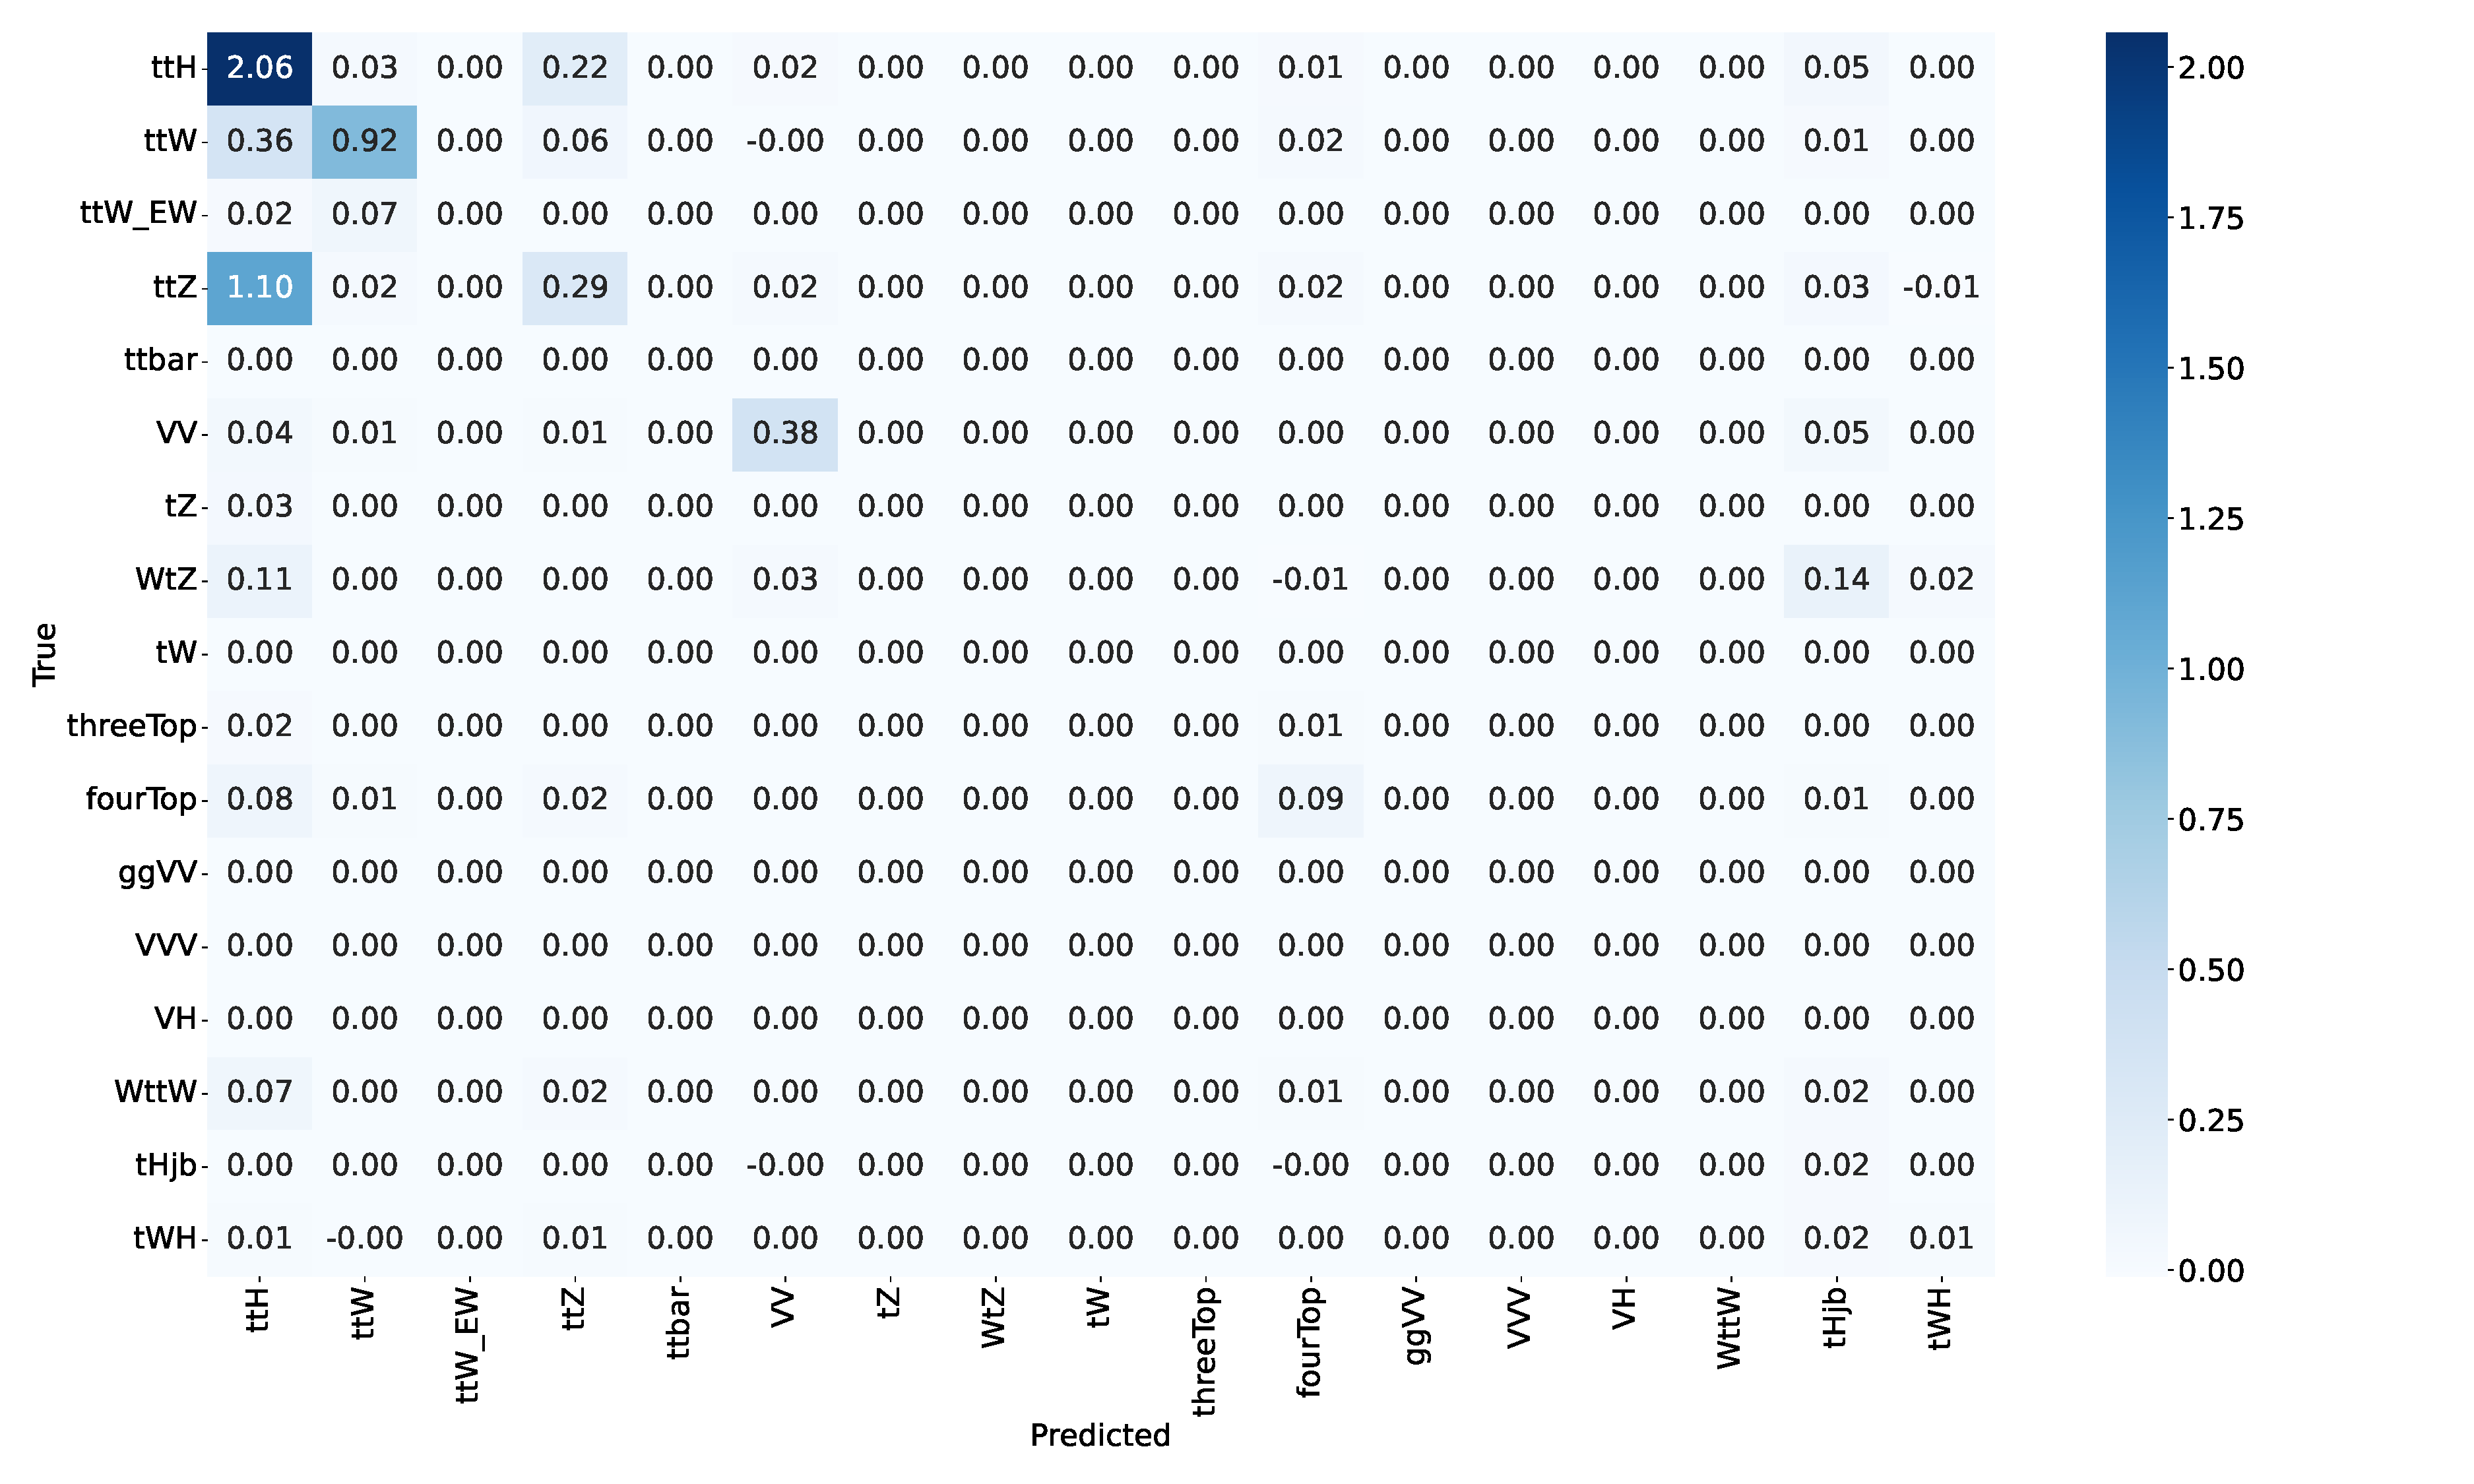
\includegraphics[trim=0.5cm 0 6cm 0, clip, width=\textwidth]{figures/ml/cm/all_argmax.pdf}
    \caption[Confusion matrix for a multi-class classification task]
    {Confusion matrix for a multi-class classification task. This confusion matrix is produced using 5-blocks
        \gls{ftt} (see \autoref{sec:ftt}) trained on the extended training set (see \autoref{sec:extended-set}). The
        $\arg\max$ classification strategy was used.}
    \label{fig:cm-muli}
\end{figure}

The confusion matrix serves as the basis for several other performance metrics, including accuracy, F1 score, and area
under the \gls{roc} curve (AUC-ROC).

\subsubsection{Accuracy: The Proportion of Correct Predictions}

Accuracy is the most intuitive performance metric. It is the proportion of the number of correctly classified examples
to the total number of examples. Accuracy is calculated trivially from the confusion matrix:

\begin{align}
    \acc  = \frac{\trace \C_{ii}}{\sum_{i=1}^\classY \sum_{j=1}^\classY \C_{ij}}\,,
\end{align}

While accuracy is straightforward and commonly used, it may not always be the most representative metric, especially in
cases where the classes are imbalanced. Consider the example of our particle physics problem where we are searching for
\tth events and suppose that 90\% of the events are background and only 10\% are signal. A naïve classifier that
always predicts the background class would achieve an accuracy of 90\%. However, such a classifier would be entirely
unhelpful for the task at hand since it fails to identify any \tth events.

Certainly, the accuracy is not entirely without value, and there are contexts where it might still be useful. Even in
imbalanced scenarios, accuracy can provide a general sense of how often the classifier is correct across both the
majority and minority classes. While it may not provide a nuanced view of performance on the minority class (such as
\tth events in our case), it still provides information on the overall hit rate of correct predictions.

Additionally, in scenarios where the cost of false positives and false negatives are roughly equivalent, or when the
class distribution in the model's operational environment matches the training data, accuracy might still be a relevant
metric. It offers a quick and easily interpretable measure of performance.

However, in the specific context of searching for rare or significant events, such as \tth in particle physics, relying
solely on accuracy can be misleading. It would typically be considered alongside other metrics that give more insight
into the performance on the class of interest. Thus, while accuracy may not be the most representative metric in such
cases, it might still hold some value as part of a broader evaluation framework.

Absolutely, let's proceed with defining precision and recall in a style consistent with what we've been working on.

\subsubsection{Precision and Recall}

Two other important metrics derived from the confusion matrix are precision and recall, which are particularly useful
when dealing with imbalanced classes.

\paragraph{Precision} is the proportion of TP to all \emph{predicted} positives. Specifically, in our case, it
is the ratio of the correctly classified \tth events, to all events classified (or misclassified) as \tth. From here on
out, we assume $y_1 = \tth$, and so the true \tth events correspond to the first row of the confusion matrix, while
predicted \tth events correspond to the first column. Precision is then given by:

\begin{align}
    \text{Precision} = \frac{\C_{11}}{\sum_{j=1}^\classY \C_{1j}}\,.
\end{align}

\paragraph{Recall} (or sensitivity) is the proportion of TP to all \emph{actual} positives. In our case, it is the ratio
of the correctly classified \tth events to all actual \tth events (which the model might have missed by classifying them
as background). Recall is given by:

\begin{align}
    \text{Recall} = \frac{\C_{11}}{\sum_{i=1}^\classY \C_{i1}}\,.
\end{align}

Precision tells us how reliable our positive predictions are,
while recall informs us how many of the actual \tth events we were able to detect. Both these metrics provide
complementary insights, and understanding the trade-off between them is essential in many real-world classification
tasks. Next, we will introduce the F1 score, a metric that combines both precision and recall to provide a balanced view
of the model's performance on both fronts.

\subsubsection{F1 score: The Balance Between Precision and Recall}

The F1 score is the harmonic mean of precision and recall, providing a balance between the two. It is calculated as:

\begin{equation}
    \text{F1 score} = 2 \cdot \frac{\text{Precision} \cdot \text{Recall}}{\text{Precision} + \text{Recall}}
\end{equation}

\subsubsection{ROC Curve and AUC: The Trade-off Between Sensitivity and Specificity}

The \gls{roc} curve is a plot of the true positive rate (recall or sensitivity) against
the false positive rate (1 - specificity) for different classification thresholds. The area under the ROC curve
(AUC-ROC) measures the classifier's ability to distinguish between classes. A perfect classifier has an AUC-ROC of 1,
while a random classifier has an AUC-ROC of 0.5. The ROC curves for the \tth and two most dominant background processes
\ttw and \ttz are shown in \autoref{fig:rocs}.

\begin{figure}[htb]
    \centering
    \begin{subfigure}{0.32\textwidth}
        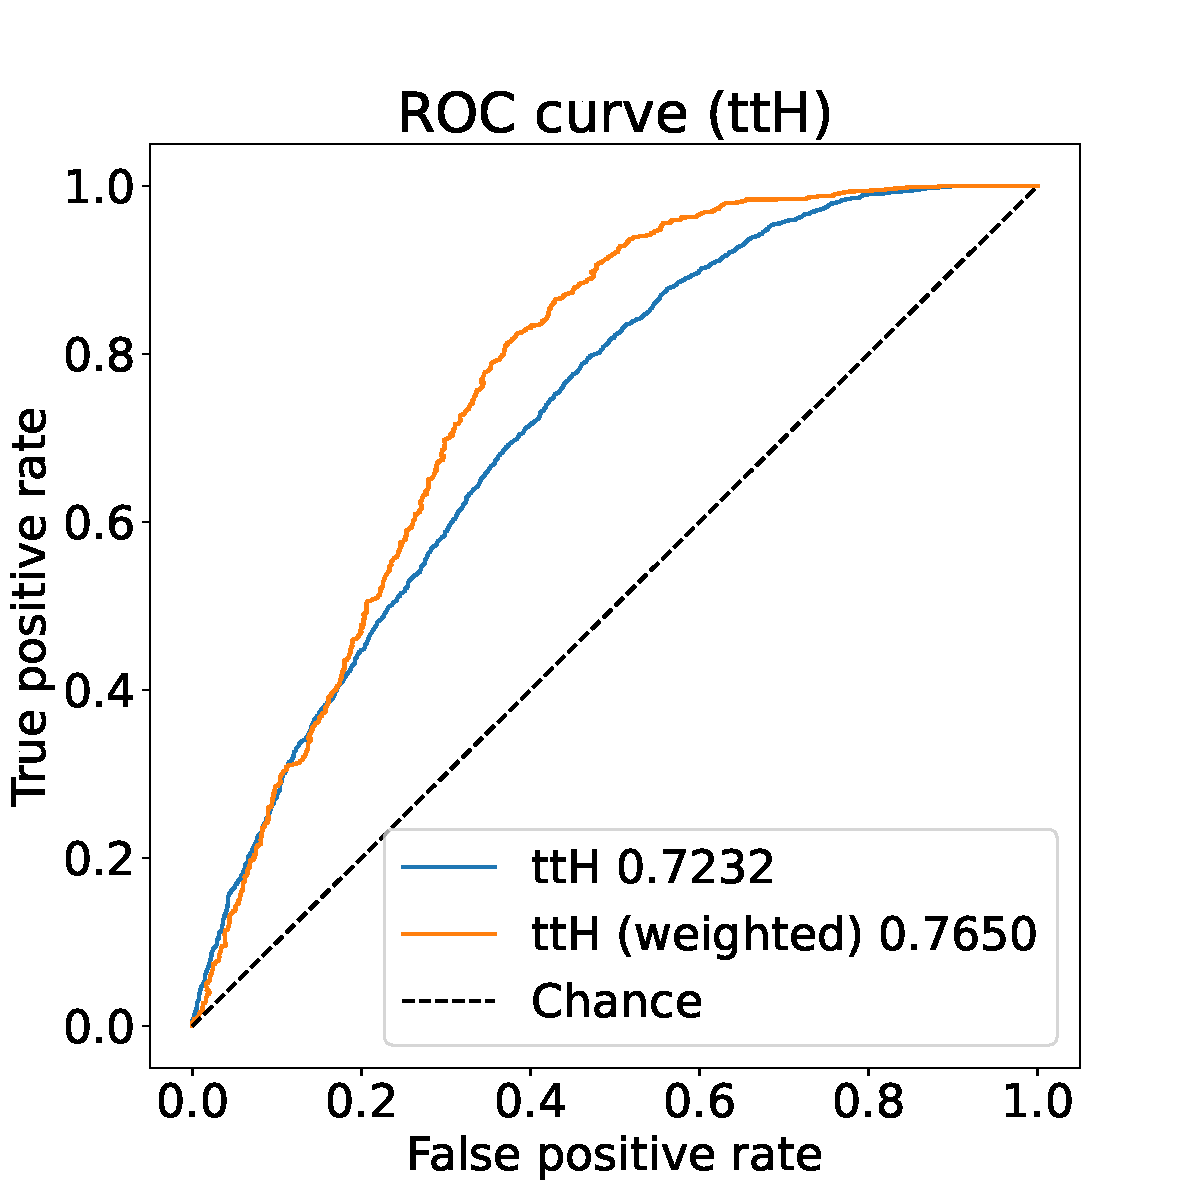
\includegraphics[width=\linewidth]{figures/ml/roc/ttH.pdf}
        \caption{\tth}
        \label{fig:roc-tth}
    \end{subfigure}
    \begin{subfigure}{0.32\textwidth}
        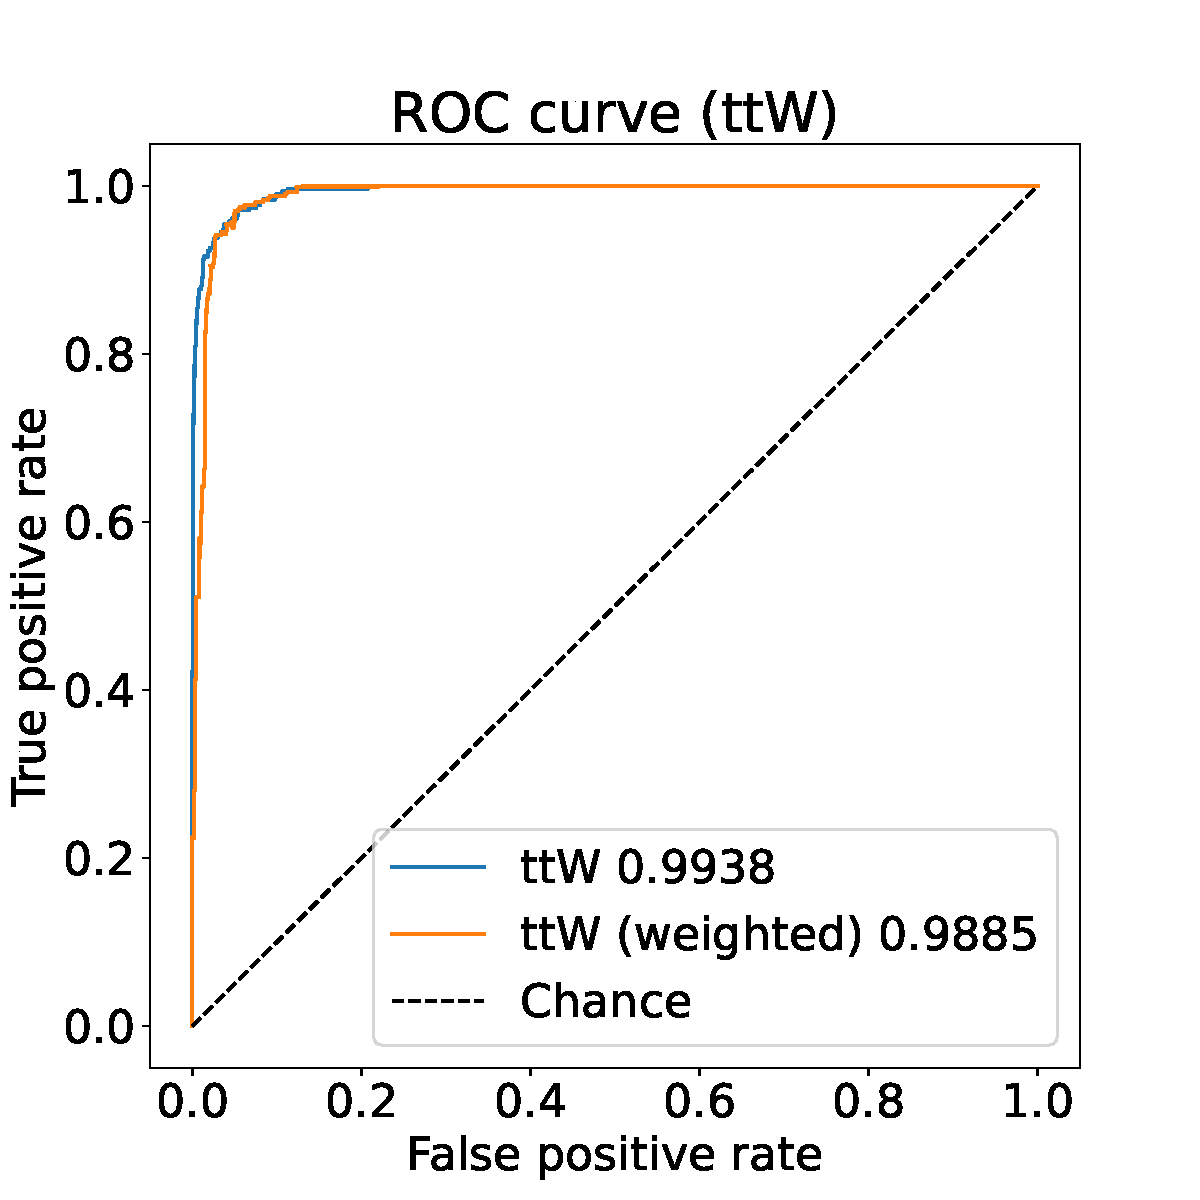
\includegraphics[width=\linewidth]{figures/ml/roc/ttW.pdf}
        \caption{\ttw}
        \label{fig:roc-ttw}
    \end{subfigure}
    \begin{subfigure}{0.32\textwidth}
        \includegraphics[width=\linewidth]{figures/ml/roc/ttZ.pdf}
        \caption{\ttz}
        \label{fig:roc-ttz}
    \end{subfigure}
    \caption[\acrshort{roc} curves for \tth, \ttz, and \ttz]
    {\gls{roc} curves for the \tth, \ttw, and \ttz computed using one versus all classification. The curves are produced
        using 5-blocks \gls{ftt} (see \autoref{sec:ftt}) trained on the extended training set (see
        \autoref{sec:extended-set}). We provide both the \glspl{roc} computed with the weighted and unweighted confusion
        matrices for completeness and comparison with the previous analysis, bet we emphasize
        that the weighted \glspl{roc} are the ones that should be used always.} \label{fig:rocs}
\end{figure}


These metrics, combined with the loss function, provide a comprehensive view of the classifier's performance and guide
the optimization process during training. They also provide a robust measure for comparing different classifiers or the
same classifier with different hyperparameters. Generally, one should examine all of these metrics to get a complete
picture of the classifier's performance.